\section{Introdução}

\subsection{Contexto}

\begin{frame}

    MOSFETs têm vantagens sobre BJT em aplicações de potência porque:
    \begin{itemize}
        \item São controlados por tensão, o que reduz consumo e complexidade no circuito de acionamento do gate;
        \item Não sofrem com acumulo de portadores minoritários quando em saturação, o que reduz o tempo de comutação;
        \item Têm coeficiente térmico positivo para R\textsubscript{on}, o que favorece a associação em paralelo
    \end{itemize}

\end{frame}

\subsection{Principais Parametros}

\begin{frame}
    
    \frametitle{V\textsubscript{blocking}}

    Máximo V\textsubscript{ds} que o dispositivo suporta, quando em bloqueio, sem que haja condução de corrente. \\
    Buscamos maximizar V\textsubscript{blocking} para aumentar a robustez do dispositivo.

\end{frame}

\begin{frame}
    
    \frametitle{R\textsubscript{on}}

    Resistência do dispositivo quando em condução. \\
    Buscamos minimizar R\textsubscript{on} para reduzir perdas em condução.

\end{frame}

\begin{frame}

    \frametitle{{R\textsubscript{on} Ideal}}

    Conforme \cite{baliga2010fundamentals},

    \begin{equation}
        R_{on, ideal} = \frac{4V_b^2}{\epsilon_s\mu{}E_c^3}
    \end{equation}

    Portanto, há um \textit{trade-off} entre o aumento da tensão de bloqueio e a redução da resistência de condução.

\end{frame}

\begin{frame}
    
    \begin{figure}[!htbp]
        \centering
        \caption{R\textsubscript{on} ideal para MOSFETs de potência em Silício}
        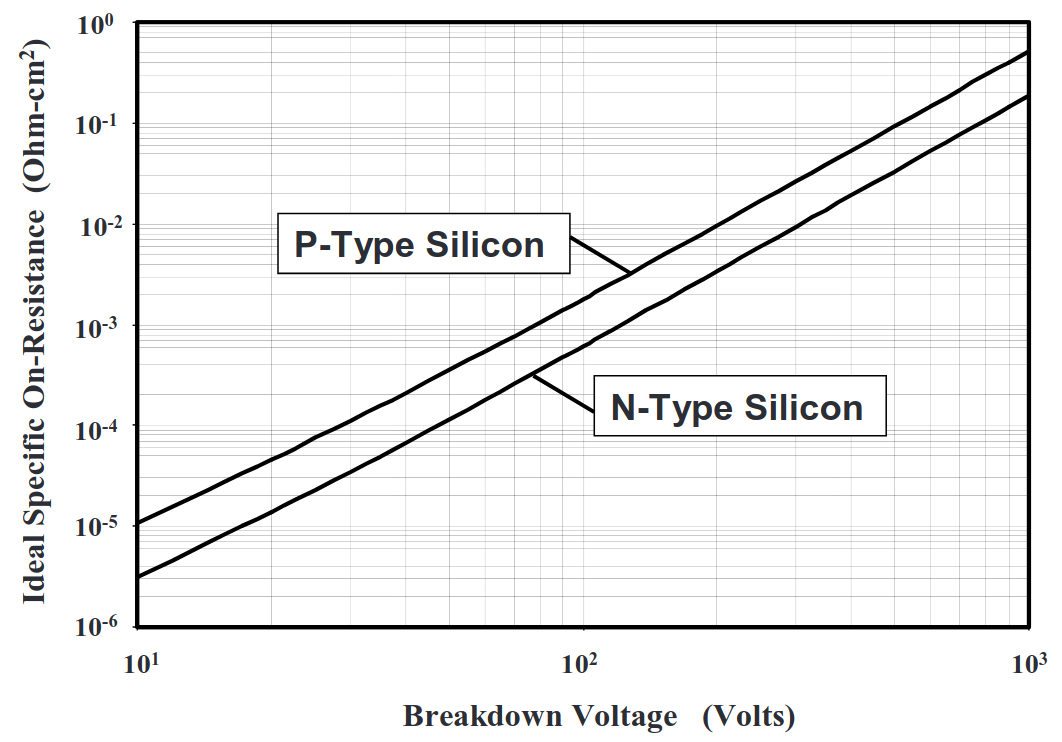
\includegraphics[scale=0.2]{imagens/ronideal.png}
     \\\small{\textbf{Fonte:} \cite{baliga2010fundamentals}}%
  \end{figure}
  
\end{frame}
